\section{RQ1: The governor sets the in-application engine time}
\label{sec:diagnosis}

\subsection{Stage attribution in a sequential application}

Each stage of a conventional sequential application was first timed
with CUDA events (float-input YOLO26n engine at 640, 1,004 images of
the train2017 verification split). The medians were 7.5\,ms
for JPEG decode, 3.9\,ms for letterbox and normalization, 0.65\,ms for
the pinned host-to-device copy, 12.4\,ms for TensorRT execution and
0.01\,ms for the output copy. With row construction and Python-side
dispatch (${\approx}1.5$\,ms), the median total is 26.0\,ms for the
OpenCV-based row path (the fallback converter of the accuracy runs is
excluded). The default governors held the CPU domain near 955\,MHz, so
these are host-stage times of a down-clocked host. A clocked repeat (domain logged at 20\,Hz, 837\,MHz
mean) reproduced every stage median within 7\% (decode 8.0\,ms,
letterbox 4.2\,ms, compute 12.9\,ms, total 26.9\,ms). Copies are
negligible on this unified-memory device, and the NMS-free output needs
no suppression. By this account the model takes about half of the
application's time and is the obvious optimization target.

The same engine, however, runs in 4.1\,ms back-to-back in
\texttt{trtexec} (zero gap, two 15\,s runs, medians 4.10 and
4.13\,ms), and the uint8-input engine of \cref{tab:dvfs} in 4.2\,ms.
On val2017, every sequential pipeline of the ladder (\cref{sec:ladder})
records a mean GPU clock of exactly 306\,MHz, the governor's floor, and
a median enqueue-to-completion time of 13.2--13.3\,ms for both input
types, $3.1$--$3.2\times$ the respective back-to-back time.

\subsection{An idle-gap sweep isolates the governor}

To isolate the governor, the uint8 engines were run in \texttt{trtexec}
with a forced idle gap between inferences, twice for 15\,s per point
(\cref{fig:dvfs}, \cref{tab:dvfs}). With locked clocks, YOLO26n's
median compute time is 4.20--4.27\,ms at every gap. With default
governors it stays at 4.2--4.3\,ms up to a 2\,ms gap, then grows to
5.5\,ms at 4\,ms, 6.8\,ms at 8\,ms and 12.4\,ms at 33\,ms. YOLO26s,
which keeps the GPU busy longer per inference, holds its 6.8\,ms up to
a 4\,ms gap and rises to 20.5\,ms at 33\,ms. The gap is host idle time:
at 33\,ms the achieved rate is about 26.7 inferences/s, with no
camera-style arrival process, and because \texttt{trtexec} pipelines
its enqueues the GPU-idle interval is shorter than the requested sleep
(\cref{tab:dvfs}). Along this axis, a host that leaves
${\approx}30$\,ms between inferences pays about $3\times$ the minimum
compute time per frame under the default governor. Camera-rate arrival
is measured in \cref{sec:stream}.

\begin{figure}[pos=t]
\centering
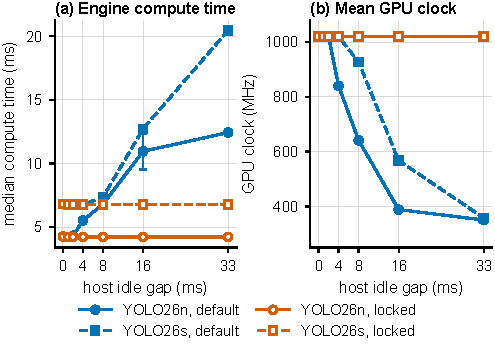
\includegraphics[width=\columnwidth]{figs/dvfs.pdf}
\caption{Median GPU compute time of the uint8 FP16 engines in
\texttt{trtexec} (left) and mean sampled GPU clock (right) versus a
forced idle gap between inferences. Mean of two 15\,s runs per point.
Default governors (blue, filled markers) versus
\texttt{jetson\_clocks} (red, open markers); circles and solid lines
show YOLO26n, squares and dashed lines YOLO26s. The
gap is host idle time (\texttt{--idleTime}), not a frame period.}
\label{fig:dvfs}
\end{figure}

\begin{table}[t]
\centering
\caption{Idle-gap sweep (\texttt{trtexec}, uint8 FP16 engines, mean of two
15\,s runs). Default governors: measured median compute time, harmonic-mean
GPU clock $\bar f$, and the prediction $G_{\max} f_{\max}/\bar f$ of
\cref{eq:gf}. ``Lock'' is the measured median with \texttt{jetson\_clocks}.
The gap axis is the requested host idle time (\texttt{--idleTime}), not a
frame period. Because \texttt{trtexec} pipelines its enqueues, the
achieved rate (last row pair) implies a mean GPU-idle interval shorter
than the requested sleep. Where the host requests 4, 8, 16 and 33\,ms,
this interval is 3.0, 5.7, 9.4 and 25.4\,ms for YOLO26n and 1.5, 4.9,
8.1 and 18.0\,ms for YOLO26s.}
\label{tab:dvfs}
\small
\setlength{\tabcolsep}{2.2pt}
\begin{tabular}{r rrrr rrrr}
\toprule
& \multicolumn{4}{c}{YOLO26n} & \multicolumn{4}{c}{YOLO26s} \\
\cmidrule(lr){2-5} \cmidrule(lr){6-9}
Gap (ms) & ms & $\bar f$ & pred. & lock & ms & $\bar f$ & pred. & lock \\
\midrule
0 & 4.25 & 1020 & 4.22 & 4.25 & 6.80 & 1020 & 6.78 & 6.80 \\
1 & 4.23 & 1020 & 4.22 & 4.22 & 6.79 & 1020 & 6.78 & 6.78 \\
2 & 4.31 & 1020 & 4.22 & 4.22 & 6.78 & 1020 & 6.78 & 6.78 \\
4 & 5.52 & 836 & 5.15 & 4.21 & 6.77 & 1020 & 6.78 & 6.78 \\
8 & 6.80 & 632 & 6.82 & 4.21 & 7.35 & 926 & 7.46 & 6.76 \\
16 & 10.95 & 355 & 12.15 & 4.21 & 12.72 & 550 & 12.57 & 6.76 \\
33 & 12.43 & 323 & 13.33 & 4.22 & 20.45 & 327 & 21.12 & 6.77 \\
\midrule
\multicolumn{9}{l}{achieved inf/s, YOLO26n: 235,\ 236,\ 169,\ 118,\ 81,\ 49,\ 27} \\
\multicolumn{9}{l}{achieved inf/s, YOLO26s: 147,\ 147,\ 147,\ 121,\ 82,\ 50,\ 27} \\
\bottomrule
\end{tabular}
\end{table}


\subsection{Validating the duty-cycle model}

\textbf{Engine time.}
\Cref{tab:dvfs} compares the measured compute time with the prediction
of \cref{eq:gf}, which uses $G_{\max}$ from the locked runs and the
harmonic-mean clock sampled during each run. Over the 14 down-clocked
sweep runs, the mean absolute error is 4.8\%, with signed per-cell
errors from $-6.7$\% (YOLO26n, 4\,ms gap) to $+11.0$\% (YOLO26n,
16\,ms gap). The largest error (23\%) occurs in one of the two
16\,ms-gap YOLO26n runs, whose median compute time differs from its
repeat's by 30\% although their harmonic-mean clocks differ by only
8\%. This suggests clock changes faster than the 20\,Hz sampling
resolves; independent measurements put the GPU clock-actuation lag
at about 5\,ms on this SoC family~\cite{kang2026emc}.

For the non-overlapped application rungs of \cref{tab:ladder},
\cref{eq:gf} overestimates the measured enqueue-to-completion time by
0.4--11.5\%. Part of this bias is expected: \cref{eq:gf} attributes all
engine time to the GPU clock, with no clock-insensitive component
(memory-bound kernels, launch overhead). The window's harmonic-mean
clock also includes host-only intervals, during which the clock is
lower. In the load-logging session, re-weighting the clock by the
driver's per-sample GPU load reduces the prefetch rungs' overestimate
from $+19$--$36$\% to $+9$--$13$\%, so much of the bias where the clock
moves is a sampling artefact of the window average. The sequential
rungs, pinned at 306\,MHz throughout, still show a $5$--$7$\%
overestimate, the cleaner estimate of the clock-insensitive share.
\Cref{eq:gf} is therefore treated as a first-order description with a
${\sim}5$\% residual, not as an exact law.

A fixed-frequency sweep avoids window averaging. With the GPU's
devfreq domain pinned at each of its eight steps (CPU and memory clocks
at their shipped settings), the uint8 engine at zero gap takes from 12.49\,ms at 306\,MHz to 4.25\,ms at
1020\,MHz (\cref{tab:fixedfreq}). A pure inverse fit $G=b/f$, with $b$
fitted by least squares, reproduces these medians with a mean absolute
error of 3.7\% but a systematic residual, positive at the floor and
negative at the top clock. The anchored form of \cref{eq:gf}
($b=G_{\max}f_{\max}$) is less accurate (6.6\% mean absolute error,
always overestimating below the top clock). The two-term fit
$G(f)=a+b/f$ removes the structure ($a=0.63$\,ms,
$b=3.63$\,GHz$\cdot$ms, mean absolute error 0.7\%, all residuals within
$\pm1.5$\%). Adding the ${\approx}0.7$\,ms launch path to the pinned
306\,MHz time reproduces the sequential pipeline's 13.2\,ms
enqueue-to-completion.

The memory (EMC) clock also scales with load on this SoC and is a
possible confound; prior work reports memory-clock effects of 11--48\%
on edge-inference latency~\cite{kang2026emc}. The sweep was therefore
rerun with three repeats per step and the EMC clock logged at
${\approx}4$\,Hz, plus two control runs with the EMC governor fully
unlocked. An attempted EMC lock did not hold; on the same SoC family,
EMC clock control is documented to fail silently on these board support
packages unless a second lock bit is asserted~\cite{kang2026emc}. The
confound is therefore controlled by measurement. The logged memory
clock is bistable across the GPU steps (\cref{tab:fixedfreq}). Fitting
$a{+}b/f$ to only the EMC-constant points changes $b$ by 2\% (3.55
versus 3.63\,GHz$\cdot$ms), and the unlocked control runs reproduce the
pinned medians within 0.4\%. The inverse trend is thus primarily a
GPU-clock effect and cannot be explained by memory-clock scaling alone.

\begin{table}[t]
\centering
\caption{Fixed-frequency sweep: the uint8 YOLO26n engine at zero idle
gap with the GPU pinned at each devfreq step (three 15\,s
\texttt{trtexec} runs per step; repeat medians agree to 1.1\%). The
memory clock is logged (constant 2133\,MHz at 306--510\,MHz,
bistable 2133--3199\,MHz from 612\,MHz up).
$G(f)=b/f$ uses the least-squares $b=3.94$\,GHz$\cdot$ms fitted to the
eight points. Anchoring $b=G_{\max}f_{\max}$ at the top point instead,
as \cref{eq:gf} does, raises the mean absolute error to 6.6\%.
The two-term fit adds
a clock-insensitive $a$. Errors are signed, (predicted $-$
measured)/measured.}
\label{tab:fixedfreq}
\small
\begin{tabular}{r rr rr}
\toprule
$f$ (MHz) & measured (ms) & $b/f$ (\%) & $a{+}b/f$ (\%) \\
\midrule
306  & 12.49 & $+3.1$ & $+0.1$ \\
408  &  9.54 & $+1.2$ & $-0.1$ \\
510  &  7.86 & $-1.7$ & $-1.3$ \\
612  &  6.48 & $-0.6$ & $+1.4$ \\
714  &  5.68 & $-2.8$ & $+0.7$ \\
816  &  5.05 & $-4.5$ & $+0.6$ \\
918  &  4.59 & $-6.5$ & $ 0.0$ \\
1020 &  4.25 & $-9.1$ & $-1.4$ \\
\bottomrule
\end{tabular}
\end{table}

\textbf{Governor operating points.}
The busy fraction $u$ of \cref{sec:sysmodel} can be estimated from
timing, but the GPU driver also reports its own load (per mille,
through sysfs). In a separate session, the eight pipeline rungs were
rerun on the first 2,000 val2017 images with this load and the GPU and
CPU clocks logged at 20\,Hz. The measured load agrees with the timing
estimate within 0.05 for every rung (the estimate is 0.01--0.05
higher) and is used for the application rungs below.

\Cref{fig:operating} plots every operating point as GPU load against
harmonic-mean clock. Whenever the governor settles clearly inside its
range (400--1000\,MHz), the load lies between 0.53 and 0.74: 0.53--0.64
for the \texttt{trtexec} sweep (timing estimate) and 0.64--0.74 for the
application rungs (measured). Two caveats apply. The two sources use
different estimators, so the lower edge cannot be separated from the
timing estimate's high bias. The 0.74 upper edge comes from a rung
settled at 993\,MHz, close to the 1020\,MHz clamp, so the true upper
threshold may lie higher. With these caveats, this is the load-band
behavior assumed in \cref{sec:sysmodel}. The sequential rungs sit at
the floor with measured loads of 0.46--0.66, at or below the observed
band's top, consistent with the governor never raising the clock (the
fixed point of \cref{sec:sysmodel}). Removing host stages from the
GPU's critical path pushes the load to the top of the band or above,
and the clock follows. Prefetch with event synchronization settles at
853\,MHz (harmonic mean) in the load-logging session and 881--891\,MHz
across the three backlog repeats; its stream-synchronized variant stays
at 655\,MHz here and at 631--694\,MHz in the blocking-sync runs of
\cref{sec:sched}. The full schedule, at a measured load of 0.87
(timing estimate 0.90), stays at 1020\,MHz.

\textbf{The floor is the only stable point observed.}
Whether a load-band controller holds a sequential pipeline at a high
clock if it starts there was tested twice: the sequential
stream-synchronized pipeline was started with locked clocks and the
default governor restored after 10\,s. At 1020\,MHz the load was only
0.35--0.36, below the band. Within 0.25\,s of the release the governor
began to step down (1020, 714, 612, 510, 408\,MHz), held 408\,MHz for
about 2.5\,s at a load of about 0.5, and reached 306\,MHz 3.3--3.4\,s
after the release, where it stayed at a load of 0.52--0.53. No run
showed a second operating point. The model does not exclude interior
equilibria (a pipeline whose load stops responding to the clock could
settle elsewhere), but for this workload the release lands at the floor
from every starting clock tested.

\begin{figure}[pos=t]
\centering
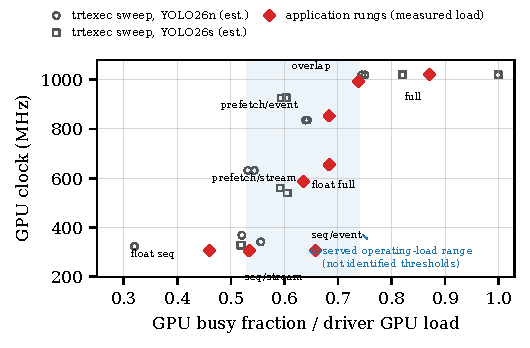
\includegraphics[width=\columnwidth]{figs/operating.pdf}
\caption{Governor operating points: GPU busy fraction or measured load versus
harmonic-mean GPU clock. Open markers: \texttt{trtexec} idle-gap
sweep, busy fraction estimated from timing. Diamonds: default-governor
application rungs (first 2,000 val2017 images), load measured by the GPU
driver. The shaded band (0.53--0.74) is the observed operating-load
range. It contains every operating point with a clock between 400
and 1000\,MHz and is not an identified pair of controller thresholds.}
\label{fig:operating}
\end{figure}

\textbf{Clock and power traces.}
In \cref{fig:traces}, both sequential variants stay at 306\,MHz,
prefetch climbs in steps from the floor and then moves between about
700 and 1020\,MHz, and the full schedule is pinned at 1020\,MHz. Input
power follows the clock. Both optimized schedules also show short power
dips whose spacing grows over the run: from about 1.9 to 4.3\,s for the
full schedule, and at longer, less regular intervals (up to about
7\,s) for prefetch. The dips were traced to Python's cyclic garbage
collector, whose pauses grow with the list of detection rows; their
effect over whole runs is quantified in \cref{sec:ladder}.

\begin{figure}[pos=t]
\centering
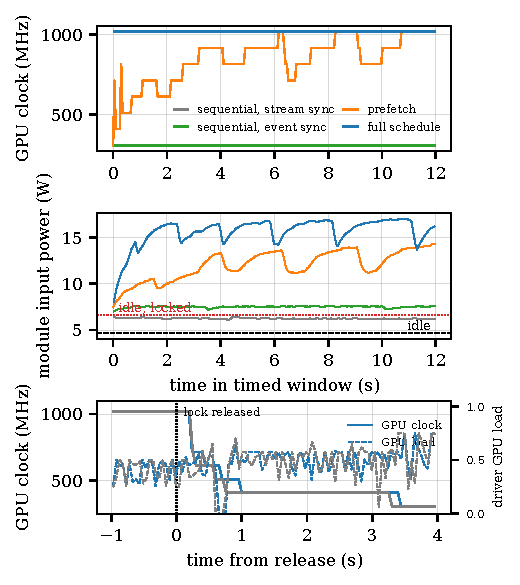
\includegraphics[width=\columnwidth]{figs/traces.pdf}
\caption{(a) GPU clock and (b) module input power during the first 12\,s
of four YOLO26n application runs on val2017 under default governors
(20\,Hz samples); the two sequential traces coincide at 306\,MHz in the
top panel. (c) The lock-then-release experiment. The sequential
pipeline is started with the GPU clock locked at 1020\,MHz, and the lock
is released at $t{=}0$ (dotted line). Clock (thick lines) and driver GPU load
(thin lines, right axis) of two repeats fall to the 306\,MHz floor within
about 3.4\,s.}
\label{fig:traces}
\end{figure}

\textbf{Answer to RQ1.}
Under the default governor, the in-application cost of a fixed engine
is set by the application's GPU duty cycle. Engine time follows the
inverse of the clock (\cref{eq:gf}). Every operating point observed
inside the governor's range sits in a GPU-load band of 0.53--0.74,
consistent with the load-band behavior of \cref{sec:sysmodel}, whose
exact thresholds are not identified. The only other observed state is
the floor. A sequential pipeline reaches it from any starting clock and
stays there, which makes its engine about $3\times$ slower than the
benchmark, a larger effect than any engine-time change produced by the
compression methods tested (\cref{sec:model}).
